\documentclass[english]{beamer}%handout,
\usepackage{babel}
\usepackage[utf8]{inputenc}
\usepackage{mathptmx}
\usepackage{amsmath,amssymb}

\usepackage{appendixnumberbeamer}
\usepackage[style=authoryear,sortcites=true]{biblatex}
\bibliography{bibliografia}
\renewcommand*{\bibfont}{\footnotesize}
\ExecuteBibliographyOptions{
  isbn=false,url=false,doi=false,eprint=false,%alldates=terse,
  firstinits=true,abbreviate=true,maxnames=2,
}
\bibparsep 0.11cm
\bibhang 0.25cm
\renewbibmacro*{title}{%
  \printfield{title}
}


\usepackage{tikz,pgfplots}
\usetikzlibrary{dateplot}
\usetikzlibrary{shapes,arrows,positioning}
%\usetikzlibrary{dateplot}  
%\usetikzlibrary{pgfplots.groupplots}






% \pgfplotsset{
%    rrbtimeseries/.style={
%         % date coordinates in=x,
%         ylabel=Temperature (K),
%         % legend style={font=\footnotesize},
%         % tick label style={font=\footnotesize},
%         % every axis x label/.style={
%         %   at={(1.3,0)},
%         %   anchor=north,
%         %   },
%         % label style={font=\footnotesize},
%         % xticklabel style= {rotate=17,anchor=north east},
% %        every axis title shift=0pt,
% %        max space between ticks=15,
%        %  every mark/.append style={mark size=6},
%        %  major tick length=0.1cm,
%        %  minor tick length=0.066cm,
%        %  very thin,
%        %  every axis legend/.append style={
%        %    at={(1.2,0)},
%        %    anchor=south east,
%        %    draw = none},
%        % legend columns = 4,
%        % unbounded coords=jump, %v>1.4
%     },

%   % rrbrs/.style={
%   %       rrbtimeseries,
%   %       width = \textwidth,
%   %       height = 0.25\textwidth,
%   %       every axis x label/.style={
%   %         at={(1.3,-1)},
%   %         anchor=north,
%   %         },
%   %       ylabel = {},  
%   %       max space between ticks=50,
%   %       every axis legend/.append style={
%   %         at={(1,-1.1)},
%   %         anchor=north east,
%   %         draw = none},
%   %       title style={font=\small,below,anchor=north,fill=white},
%   %   },
%  }




\pgfplotsset{
   timeseries/.style={
%        date coordinates in=x,
        ylabel=Temperature (K),
        legend style={font=\footnotesize},
        tick label style={font=\footnotesize},
        every axis x label/.style={
          at={(1.3,0)},
          anchor=north,
          },
        label style={font=\footnotesize},
        xticklabel style= {rotate=17,anchor=north east},
%        every axis title shift=0pt,
%        max space between ticks=15,
        every mark/.append style={mark size=6},
        major tick length=0.1cm,
        minor tick length=0.066cm,
        very thin,
        every axis legend/.append style={
          at={(1.2,0)},
          anchor=south east,
          draw = none},
       legend columns = 4,
    },
    rd/.style={
        timeseries,
        % every axis x label/.style={
        %   at={(1.3,-1)},
        %   anchor=north,
        %   },
        label style={font=\footnotesize},
        ylabel = {},
        width=\textwidth,
        height=3.5cm,   
        max space between ticks=50,
        every axis legend/.append style={
          at={(1,-1.1)},
          anchor=north east,
          draw = none},
%        title style={font=\small,below, at={(0.7,1.7)},anchor=north},
    }
}


%        unbounded coords=jump, %v>1.4
%        unbounded coords=discard, %v>1.4


%http://tex.stackexchange.com/questions/46422/axis-break-in-pgfplots

%http://tex.stackexchange.com/questions/52409/insert-a-separate-mark-inside-a-pgfplots-graph

\usepackage[overlay]{textpos}


\mode<presentation>
{
  \usetheme{Madrid}
  \setbeamertemplate{headline}{
    \begin{beamercolorbox}{section in head/foot}
      \insertnavigation{\paperwidth}
    \end{beamercolorbox}
  }
  \setbeamercovered{transparent}
  \beamertemplatenavigationsymbolsempty
}


\mode<handout>
{
  \usepackage{pgfpages}
  \pgfpagesuselayout{8 on 1}[a4paper,border shrink=5mm]
  \setbeamercolor{background canvas}{bg=black!5}
  \usetheme{Boadilla}
  \useinnertheme{default}
  \usecolortheme{dove}
}


%\usepackage{hyperref}



\newcommand{\acro}[1]{\textsc{\lowercase{#1}}}








%------------- portada -----------

\title%
   [Multiresolution time series DBMS]%
   {A Model for a Multiresolution \\ Time Series Database System}

\author[Escobet \and Llusà \and Vila]{%
  Teresa Escobet-Canal \and Aleix Llusà-Serra \and Sebastià Vila-Marta}

\institute[DiPSE--UPC]
{
  {\large Universitat Politècnica de Catalunya (UPC)} \\
  Department of Electronic Systems Design and Programming (DiPSE) \\

  {\tiny Av.~Bases de Manresa 61--73, 08242 Manresa, \scshape ES-CT}

  {\tiny teresa.escobet@upc.edu \quad  aleix@dipse.upc.edu \quad sebas@dipse.upc.edu}

}


\date[\acro{AIKED}' 13, Cambridge, UK]
{\acro{AIKED}' 13, Cambridge, UK. February 20--22, 2013}


\subject{aiked' 13}
\keywords{time series; data model; database systems; monitoring systems}

\begin{document}


\begin{frame}[plain]
 
 \titlepage

\end{frame}


\section*{Contents}
\begin{frame}{Contents}
  \tableofcontents
\end{frame}


\section{Introduction}
\begin{frame}{Índex}
  \begin{enumerate}
  
  \item Introducció
    \begin{enumerate}
    \item Sistema de monitoratge
    \item Sèries temporals
    \item Sistemes de Gestió de Bases de Dades (SGBD)
    \end{enumerate}
    
  \item SGBD RRDtool 
    
  \item Model de dades Round Robin (RRD)
    
  \item Implementació de referència del model RRD
    
  \item Conclusions
    
  \item Treball futur
    
  \item Referències
\end{enumerate}
\end{frame}




\begin{frame}{Introducció. Sistema de monitoratge: situació del problema}

  \begin{itemize}
  \item \emph{Supervisory Control And Data Acquisition} (SCADA). 
  \item Adquisició de dades $\Rightarrow$  monitoratge:

    \begin{itemize}
    \item Moltes dades: només una petita part poden ser observades en línia.
    \item Volem extreure coneixement  de les dades  $\Rightarrow$ sèries temporals.
    \end{itemize}
  \end{itemize}

  \begin{center}
    \scriptsize 
    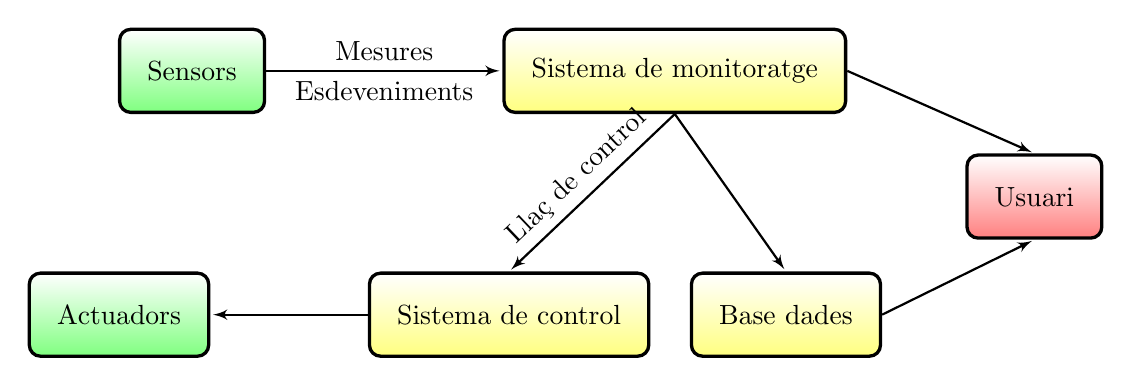
\begin{tikzpicture}[node distance=0.5cm]  
      \tikzset{
        mynode/.style={rectangle,rounded corners,draw=black, 
          very thick, inner sep=1em, minimum size=3em, text centered,
          groc},
        myarrow/.style={->, >=latex', shorten >=1pt, thick},
        mylabel/.style={text width=7em, text centered},
        groc/.style={top color=white, bottom color=yellow!50},
        verd/.style={top color=white, bottom color=green!50},
        roig/.style={top color=white, bottom color=red!50},
      }  

      \node[mynode]                                       (monitor)   {Sistema de monitoratge};  
      \node[mynode, below right=2cm and -2cm of monitor]  (bd)        {Base dades}; 
      \node[mynode, below=2cm of monitor, left=of bd]     (control)   {Sistema de control}; 
      \node[mynode, roig, below right=0.5cm and 1.5cm of monitor] (usuari)    {Usuari};  
      \node[mynode, verd, left=2cm of control]            (actuador)  {Actuadors};
      \node[mynode, verd, left=3cm of monitor]            (sensor)    {Sensors};  
      
      
      \draw[myarrow] (monitor.east) --   (usuari.north);	
      \draw[myarrow] (bd.east) --   (usuari.south);
      \draw[myarrow] (sensor.east) --   (monitor.west) 
         node [above,midway] {Mesures}
         node [below,midway] {Esdeveniments};
      \draw[myarrow] (control.west) -- (actuador.east);
      \draw[myarrow] (monitor.south) -- (bd.north);
      \draw[myarrow] (monitor.south) -- (control.north)
         node [above,sloped,midway] {Llaç de control};
      
    \end{tikzpicture} 
  \end{center}


\textbf{Objectiu:} Dissenyar un model pels SGBD dels sistemes de monitoratge.
\end{frame}




\begin{frame}{Introducció. Sèries temporals: estat actual.}

\begin{itemize}
\item Són co\l.leccions d'observacions cronològiques de magnituds.
\item Són de gran dimensió (gran nombre de punts).
\item Són de naturalesa contínua i numèrica.
\item Ofereixen representació, indexat, cerca de similituds,
  segmentació, visualització, extracció coneixement (predicció, cerca
  de patrons\ldots).
\end{itemize}

La recerca s'ha incrementat en la darrera dècada: és important
disposar d'esquemes de representació més efectius i eficients,
\parencite{fu11}:
\begin{itemize}
\item Reduir la dimensió: mostreig, \parencite{astrom69}, interpolació
  lineal amb PLR, \parencite{keogh97}, mitjana de segments amb PAA,
  \parencite{keogh00}, etc.
\item Indexar: iSAX, \parencite{keogh08:isax}, T-Time,
  \parencite{assfalg08:ttime}, etc.
\end{itemize}


\end{frame}


\begin{frame}{Introducció. SGBD: què són?}


Una base de dades és un contenidor informàtic per a una co\l.lecció de dades.

\begin{itemize}
\item El model d'una bases de dades, que és el model matemàtic a on es
  descriu teòricament l'estructura de les dades, per exemple el model
  relacional o model Round Robin.

\item El sistema de gestió de bases de dades, que és la implementació
  d'un model de dades, per exemple postgresql o
  RRDtool. 

\item La base de dades, que és una instància d'un sistema de gestió de
  bases de dades, per exemple la base de dades dels estudiants o la
  base de dades de la temperatura de l'escola.
\end{itemize}


Els SGBD habituals són els relacionals,  disposen d'un model matemàtic consolidat.

\end{frame}



\begin{frame}{Introducció. SGBD per sèries temporals: què aporten?}

Què no aporten els SGBD tradicionals?:
\begin{itemize}
\item SGBD relacionals permeten \emph{bitemporal data}: \emph{created} i  \emph{modified}, però dificulten operacions temporals de les sèries temporals. 

\item Les mesures són camps numèrics individuals i no un sol conjunt.

\item Cerca aproximada per les sèries temporals; en els SGBD és exacta.

\item Estructures amb dimensió temps: \emph{Time Series Database Systems}. 
\hspace{1cm}-- Extensió de tipus i operacions \parencite{stonebraker86}.

\end{itemize}

\medskip

Els TSDS habituals no consideren els sistemes de monitoratge:
\begin{itemize}
\item Temps de les mesures no regular (mostres no equi-espaiades).
\item Tractament de valors desconeguts.
\item L'ordre temporal és essencial. Valor i temps són inseparables.
\end{itemize}

\medskip

RRDtool: TSDS per a monitors de sèries temporals.


\end{frame}

%%% Local Variables: 
%%% mode: latex
%%% TeX-master: "presentacio"
%%% End: 


\section{Time Series}





\begin{frame}{Time Series}
  Una base de dades TSMS és un contenidor informàtic d'una
  sèrie temporal que prové d'un monitoratge d'una variable mesurada en
  diferents instants de temps.

  \begin{enumerate}

  \item Measure $m=(v,t)$. Value measured in a time instant.
    \begin{itemize}
    \item The time value defines the canonical order between measures
    \end{itemize}

  \item Time series $S=\{m_0,\ldots,m_k\}$. Sequence of measures.
    \begin{itemize}
    \item Same phenomena
    \item No repeated time values
    \item Regular time series when measures are equi-spaced.
    \end{itemize}

  \end{enumerate}

\end{frame}


%%% Local Variables: 
%%% ispell-local-dictionary: "british"
%%% mode: latex
%%% TeX-master: "presentacio"
%%% End: 


\section{The Multiresolution data model}

\section{Model}

\acro{MTSMS}
\acro{MTSM}


La definició del model s'estructura en dues parts:

\begin{itemize}
\item Un model pels (SGST)  que defineix mesura i sèrie temporals.
\item Un model pels (SGSTM) que defineix buffer, disc i subsèrie
  resolució, el qual treballa sobre el model de SGST.
\end{itemize}

\todo{sobre tres nivells}
A l'estat de l'art s'ha d'haver explicat els tres nivell de model de dades segons Date i deixar clar aquí que nosaltres definim un model pel segon nivell: nivell de model lògic. Els models lògics modelen les dades, en canvi els models conceptuals modelen la realitat, Fabian Pascal posa d'exemple conceptual el model E/RM.


Objectius:

En el model de SGST s'observen algunes patologies que poden presentar les sèries temporals. El model de SGSTM soluciona algunes d'aquestes patologies:

\begin{itemize}
\item Regularitza les sèries temporals
\item Tracta i validar les sèries temporals: gestiona els casos de dades errònies o desconegudes i marca quan hi ha valors erronis.
\item És una solució de compressió per a quantitats enormes de dades
\end{itemize}


Però el model de SGSTM també es pot fer servir per altres aplicacions:

* Regularitzar en línia (temps real) una sèrie temporal en diferents períodes de mostreig

* Tenir unes vistes (consultes) a punt (ja processades) amb diferents resolucions d'una sèrie temporal

* Comprimir per decimació (downsampling) o bé farcir forats (reconstrucció del senyal)




\section{Time series preliminaries}
\label{sec:model:preliminaries}

% In this section we introduce some background concepts and the
% nomenclature which we will use later.  First we define the main
% objects of a \acro{MTSMS} which are measures and time series.

% A \emph{measure} is a value measured in a time instant. More formally
% it is a tuple $(v,t)$ where $v$ is the value of the measure and $t \in
% \mathbb{R}$ is the time instant of measurement.  The values of a time
% series can be of any type. For simplicity examples are presented with
% integers or real numbers but can also be strings or vectors.  Let $m =
% (v,t)$ be a measure, $v$ is written as $V(m)$ and $t$ is written as
% $T(m)$.

% The time value defines the canonical order between measures.  Let $m =
% (v_m, t_m)$ and $n = (v_n, t_n)$ be two measures, then $m\geq n$ if
% and only if $t_m\geq t_n$.

% A \emph{time series} is sequence of measures of the same phenomena
% that are ordered in time.
% \begin{definition}[Time series]
%   A \emph{time series} $S$ is a a set of measures of the same
%   phenomena $S = \{m_0, \ldots, m_k\}$ without repeated time values
%   $\forall i,j: i\leq k, j\leq k, i\neq j : T(m_i)\neq T(m_j)$. Given
%   a time series $|S|$, we note its size by $|S|=k+1$. Observe that,
%   because measures in $S$ are of the same phenomena, the type of $S$
%   values is homogeneous.
% \end{definition}

% The order defined by measures implies a total order in a time
% series. As a time series is a finite set, if it is not empty it has a
% maximum and a minimum.  Let $S=\{m_0,\ldots,m_k\}$ be a time series
% and $n\in S$ be a measure. The time series' maximum is $n=\max(S)$ if
% and only if $\forall m \in S: n \geq m $.  Similarly, the time series'
% minimum is $n=\min(S)$ if and only if $\forall m \in S: n \leq m$.

% Given the order defined by time, in a time series we define the
% sequence interval following \cite{last:keogh,last:hetland}.  Let
% $S=\{m_0, \ldots, m_k\}$ be a time series. We define the subset
% $S(r,t] \subseteq S$ as the time series $S(r,t]=\{m\in S | r<T(m)\leq
% t\}$, where $r$ and $t$ are two instants in time.  We also define the
% subset $S(r,+\infty)\subseteq S$ as the time series $S(r,+\infty) =
% \{m\in S | r< T(m) \leq T(\max(S))\}$ and the subset
% $S(-\infty,t)\subseteq S$ as the time series $S(-\infty,t) = \{m\in S
% | T(\min(S))\leq T(m) < t\}$.

% The time order in time series also implies the sequence concept of
% next and previous measure.  Let $S=\{m_0, \ldots, m_k\}$ be a time
% series and $l\in S$ and $n$ be two measures. We define the next
% measure of $n$ in $S$ as $l=\nex_S(n)$ where $l =
% \min(S(T(n),+\infty))$. We define the previous measure of $n$ in $S$
% as $l=\prev_S(n)$ where $l = \max(S(-\infty,T(n)))$.

% Let $S$ be a time series, $t$ be a time instant and $\delta$ be a
% time duration, then the time series' measures can be located in the
% time interval $i_0=[t, t+\delta]$ and its multiples $i_j=[t+j\delta,
% t+(j+1)\delta]$ for $j=0,1,2,\ldots$. When time series' measures are
% equally spaced we say it to be regular.
% \begin{definition}[Regular time series]
%   Let $S=\{m_0,$ $ldots,$ $m_k\}$ be a time series and $\delta$ a time
%   duration. $S$ is regular if and only if $\forall m \in
%   S(T(\min(S),+\infty):T(m) - T(\prev_S(m)) = \delta$.
% \end{definition}









\section{Multiresolution model}
\label{sec:MTSMS}

The \acro{MTSMS} are \acro{TSMS} that store time series with a lossy
compression approach, that is some information is selected and spread in
different time resolutions. The \acro{MTSMS} model is based on the
concepts of measures and time series as defined in
Section~\ref{sec:model:preliminaries}.


The multiresolution concept comes from thoroughly analysis of the
RRDtool \cite{rrdtool} \acro{TSMS}. Our objective is to formalise its
essential parts into an abstract model, where what we call
multiresolution plays a main role, and to include more genericity in
order to describe \acro{MTSMS} as fully \acro{TSMS}. Then we will be
able to apply these systems to other applications.



A \acro{MTSMS} stores multiresolution time series where each has a
multiresolution schema as shown in Figure~\ref{fig:model:mtsdb}. A
multiresolution time series is a collection of resolution subseries
which temporarily accumulate measures in a buffer in order to select
some information and finally store it in a disc. The information
selection process changes the time intervals between measures to
compact information by aggregating the time series attributes. 

\begin{figure}[tp]
  \centering
  \input{imatges/mtsms-arquitectura_interna.tex}
  \smallskip
  \caption{Architecture of \acro{MTSMS} model}
  \label{fig:model:mtsdb}
\end{figure}


In this way, the original time series gets stored spread in the discs,
each with a different time resolution and attribute aggregation.
Discs are size bounded so they only contain a fixed amount of
measures. When a disc becomes full it discards a measure. Thus,
multiresolution database is bounded in size and the time series gets
stored in pieces, that is time subseries.

Regarding to operations, \acro{MTSMS} structure needs operators to
change the time intervals between measures and to select
attributes. Mainly, these operators are measure additions and time
series consolidations which some functionality is delegated to operators called 
attribute aggregate functions.
 Most of these operators
are attribute aggregate functions and consolidation actions.
the operations to
create a multiresolution database, to add measures, and to consolidate
time series.
 Attribute aggregate functions are required but not linked
to the model.\todo{}

Following we define the \acro{MTSMS} model by: (i) four basic
structure model elements ---buffer, disc, resolution subserie, and
multiresolution time series--- with its structure operators, (ii) the
operations to change and consult a multiresolution schema, and (iii)
the attribute aggregate functions.



\subsection{Structure}



\subsection{operations}




\section{The proposed data model}



Regarding to operations, \acro{MTSMS} structure needs operators to
change the time intervals between measures. Most of these operators
are attribute aggregate functions and consolidation actions.

In what follows we describe the basic \acro{MTSMS} model centered in:
(i) the four basic data model elements ---buffer, disc, resolution
disc, and multiresolution database---, and (ii) the operations to
create a multiresolution database, to add measures, and to consolidate
time series. Attribute aggregate functions are required but not linked
to the model. They are defined in the
Section~\ref{sec:model:interpolador}.

A \emph{buffer} is a container for a regular or a no-regular time
series. The buffer objective is to regularise the time series using a
predetermined step and an attribute function. We name
\emph{consolidation} to this action.
\begin{definition}[Buffer]
  A \emph{buffer} is defined as the tuple $(S,\tau,\delta,f)$ where
  $S$ is a time series, $\tau$ is the last consolidation time,
  $\delta$ is the duration of the consolidation step and $f$ is an
  attribute aggregate function.

  An empty buffer $B_{\emptyset} = (\emptyset,t_0, \delta, f)$ has an
  empty time series, an initial consolidation time $t_0$ and
  predetermined $\delta$ and $f$. From the $B_{\emptyset}$ all the
  consolidation time instants can be calculated as $t_0+i\delta,
  i\in\mathbb{N}$.
\end{definition}

Operator \emph{addBuffer} adds a measure to its time series:
$\text{addBuffer}: B = (S,\tau,\delta,f) \times m \mapsto
(S',\tau,\delta,f)$ where $S' = S \cup \{m\} $.

A buffer is ready to consolidate when the time of some measure is
bigger than the buffer's next consolidation time.  Let
$B=(S,\tau,\delta,f)$ be a buffer and $m=\max(S)$ the maximum measure,
$B$ is ready to consolidate if and only if $T(m) \geq \tau+\delta$.
The consolidation of $B$ in the time interval $i=[\tau,\tau+\delta]$
results in a measure $m'=(v,\tau+\delta)$ where $m'=f(S,i)$ and $f$ is
an attribute aggregate function $f$. Operator \emph{consolidateBuffer}
consolidates a set of measures and removes the consolidated part of
the time series from the buffer. Usually consolidateBuffer is only
applied to the present consolidation interval and it is defined as
follows: $\text{consolidateBuffer}: B=(S,\tau,\delta,f) \mapsto B'
\times m' $ where $ B'= (S',\tau+\delta,\delta,f)$, $S' = S$ and $m' =
f(S,[\tau,\tau+\delta])$. When historic data is not needed anymore the
consolidated buffer measures can be removed applying $S' =
S(\tau+\delta,\infty)$.

A \emph{disc} is a finite capacity measures container. A time series
stored in a disc has its cardinal bounded. When the cardinal of the
time series is to overcome the limit, some measures need to be
discarded.
\begin{definition}[Disc]
  A \emph{disc} is a tuple $(S,k)$ where $S$ is a time series and
  $k\in\mathbb{N}$ is the maximum allowed cardinal of $S$.  An empty
  disc $D_{\emptyset} = (\emptyset,k)$ has an empty time series and
  the $k$ maximum cardinal allowed.
\end{definition}

The cardinal of the times series is kept under control by the add
operator, $\text{addDisc}:D=(S,k)\times m\mapsto (S',k)$ where 
$$
S' = \begin{cases}
  S\cup\{m\}                 & \text{if } |S|<k  \\
  (S-\{\min(S)\}) \cup \{m\} & \text{otherwise}
\end{cases}  
$$

A \emph{resolution disc} is a disc which stores a regular time
series. It is composed of a buffer, that contains the partial time
series to be regularised, and a disc, that contains the regularised
time series.
\begin{definition}[Resolution disc]
  A \emph{resolution disc} is a tuple $(B,D)$ where $B$ is a buffer
  and $D$ is a disc.  An empty buffer and empty disc imply an empty
  resolution disc $R_{\emptyset} = (B_{\emptyset},D_{\emptyset})$.
\end{definition}
 
The operators of a resolution disc extend the buffer and disc ones:
(i) The addition of a measure to the buffer of the resolution disc,
$\text{addRD}:R=(B,D) \times m \mapsto R'$ where $R'= (B',D)$, and
$B'= \text{addBuffer}(B,m)$; (ii) The consolidation of the resolution
disc by consolidating its buffer and adding the consolidation measure
to its disc, $\text{consolidateRD}:R=(B,D) \mapsto R'$ where $R'=
(B',D')$ and $(B',m') = \text{consolidateBuffer}(B)$ and $D'=
\text{addDisc}(B,m')$.
% \]

A \emph{multiresolution database} is a set of resolution discs which
share the input of measures, that is they store the same time
series. A time series is stored regularised and distributed with
different resolutions in the various resolution discs, as it was shown
in the Figure~\ref{fig:model:mtsdb}.
\begin{definition}[Multiresolution Database]
  A \emph{Multi\-re\-solution Database} is a set of resolution discs
  $M=\{R_0, \dots, R_d\}$.  An empty multiresolution database has
  empty resolution discs $M_{\emptyset}=\{R_{0_\emptyset}, \dots,
  R_{d_\emptyset}\}$.
\end{definition}

We define the addition of a measure to every resolution disc as
$\text{addMD} : M=\{R_0, \dots, R_d\} \times m \mapsto \{R'_0, \dots,
R'_d\}$ where $R'_i=\text{addRD}(R_i,m)$.

The consolidation of all resolution discs can be defined as follows:
$\text{consolidateMD}: M=\{R_0, \dots, R_d\} \mapsto \{R'_0, \dots,
R'_d\}$ where
$$ 
R'_i = \begin{cases}
  \text{consolidateRD}(R_i) & \text{if } R_i \text{ ready to consolidate} \\
  R_i                       & \text{otherwise}
\end{cases}
$$.


\subsection{Attribute aggregate function}
\label{sec:model:interpolador}

When a buffer is consolidated we summarise the time series information
using an attribute aggregate function.  Let $S$ be a time series and
$t_0$ and $t_f$ two time instants, an attribute aggregate function $f$
calculates a measure that summarises the measures of $S$ included in
the time interval $i=[T_0,T_f]$:
\begin{align*}
f&:S=\{m_0,\ldots,m_k\} \times [T_0,T_f] \mapsto m'
\end{align*}

To summarise a time series we can use different attribute aggregate
functions.  For instance, we can calculate an statistic indicator of
the time series such as the average or we can apply a more complex
digital signal processing operation, \cite{zhang11}.

Below there are some examples. Let $S'=S(T_0,T_f]$. Then:
\begin{itemize}
\renewcommand{\labelitemi}{--}
\item maximum$^d$: $S \times i \mapsto m'$ where $V(m') =
  \max_{\forall m \in S'}(V(m))$. It summarises $S'$ with the maximum
  of the measure values.
\item last$^d$: $S \times i \mapsto m'$ where $V(m') = \max(S')$. It
  summarises $S'$ with the maximum measure.
\item arithmetic mean$^d$: $S \times i \mapsto m'$ where $V(m') =
  \frac{1}{|S'|} \sum\limits_{\forall m\in S'} V(m)$. It
  summarises $S'$ with the mean of the measure values.
\end{itemize}

% With reference to data validation, attribute aggregate functions
% can cope with this process. When data has not been captured or has
% been captured erroneously, it must be treated as unknown data.
% \begin{itemize}
% \item When data has not been captured it is unknown by nature. For
%   example, we try to capture data from a sensor and there is no
%   response.
% \item When data is erroneously it must be marked as unknown. For
%   example, we capture data from a sensor but it responses in a not
%   reasonable time or we capture data that is clearly outside a
%   reasonable limits.
% \end{itemize}
% As a consequence, attribute aggregate functions deals with these two
% subprocesses: treating unknown data and marking data as
% unknown. Following with real numbers example, we extend the
% domain with a value that means 'unknown', let this unknown value be
% represented by the improper element infinity ($\infty$).

% An attribute aggregate functions treating unknown
% data is a one that can calculate a result when there are unknown
% values in the original time series, $f^u: S \times i \mapsto m'$ where
% $\exists m \in S: V(m)=\infty$. Although from a strict point of view
% operating with unknown data makes unknown result, aggregate functions
% are free to calculate whatever is needed such as time series analysis
% does with data reconstruction.

% For example, arithmetic mean$^{d}$ aggregate function returns
% $V(m')=\infty$ if $\exists m \in S: V(m)=\infty$.  We can define a new
% mean function, based on the original arithmetic mean$^{d}$ aggregate,
% that naively treats unknown values by keeping the
% known mean; in other words, it ignores unknown values found in the time
% interval: arithmetic mean$^{du}$: $S \times i \mapsto m'$ where $m' =
% \text{arithmetic mean}^{d}(S'',i)$ and $S''= \{m''\in S':V(m'')\neq
% \infty\}$.
% % ignore$^{u}$: $S \mapsto S'$ where $S'= \{m''\in S':V(m'')\neq
% % \infty\}$,
% % arithmetic mean$^{du}$: $S \times i \mapsto m'$ where $m' =
% % \text{arithmetic mean}^{d}(\text{ignore}^u(S),i)$.

% An attribute aggregate functions marking data as unknown is a one
% that can give unknown value as the resulting measure's value, $f^{mu}:
% S \times i \mapsto m'$ where $V(m')\in \mathbb{R}\cup\{\infty\}$.

% For example, we can define a maximum aggregate, based on the
% maximum$^d$ aggregate, that returns unknown if there is a
% measure's value bigger than 2:  maximum$^{dmu2}$: $S \times i
% \mapsto m'$ where $V(m') = 
% \begin{cases}
%   \infty &\text{if }  m''>2\\
%   m'' & \text{else }
% \end{cases}$ and $m''=\text{maximum}^d(S,i)$.

% %Per exemple definim un termini, si les dades estan més espaiades que 2 es marca com a desconeguda

In the design of the attribute aggregate function we can interpret a
time series in different ways, that is what we call the representation
of a time series. \citeauthor{last:keogh}, \cite{last:keogh}, cite
some possible representations for time series such as Fourier
transforms, wavelets, symbolic mappings or piecewise linear
representation. The last one is very usual due to its simplicity,
\cite{keogh01}.

Time series representations can be taken into account when computing
with the measures of the time series.  For example, a maximum
attribute aggregate function may give different values if we consider
a linear or a constant piecewise representation.

Following we show a possible family of attribute aggregate functions
for time series represented by a staircase function, that is with a
piecewise constant representation.  We define a new representation for
time series named \emph{zero-order hold backwards} (zohe). This
representation holds back each value until the preceding value. 
RRDtool, \cite{lisa98:oetiker}, has a similar aggregate function.

Let $S=\{m_0,\ldots,m_k\}$ be a time series, we define
$S(t)^{\text{zohe}}$ as its continuous representation along time $t$:
$\forall t \in \mathbb{R} ,\forall m \in S:$
\begin{equation}
 S(t)^{\text{zohe}} =  
\begin{cases}
  \infty & \text{if } t > T(\max S) \\
  V(m)   & \text{if } t\in (T(\prev_S m),T(m)]
\end{cases}
\label{eq:zohe}
\end{equation}


In conclusion, we can define many attribute aggregate functions and
thus no global assumptions can be made about them. Each user has to
decide which combination of aggregation and representation fits better
with the measured phenomena.  Therefore, \acro{MTSMS} must allow to
define user aggregate functions.







%%% Local Variables:
%%% TeX-master: "main"
%%% ispell-local-dictionary: "british"
%%% End:

% LocalWords:  genericity


\section{Multiresolution Example}
\section{Example}

Next we show an example database for a real time series data.  In a
distributed sensor monitoring system temperature data has been
captured from various sensors. In this example we focus on data from
one sensor.  \todo{citar article isense}

Original data is shown in figure~\ref{fig:exemple:original} for a
period of one year and a half, from 29th April 2010 to 18th October
2011.  The time series is plotted interpolating linearly its measures.
In this plot we can see that there is missing data and some outlying
observations, and there are 146709 stored values.


\begin{figure}[tp]
  \centering
  \usetikzlibrary{dateplot}    
\begin{tikzpicture}
    \begin{axis}[
        date coordinates in=x,
%        xticklabel={\pgfcalendar{tickcal}{\tick}{\tick}{\pgfcalendarshorthand{m}{.}}},
        xticklabel={\pgfcalendarmonthshortname{\month} \year},
        xticklabel style= {rotate=15,anchor=east},
        xlabel=Time,
        ylabel=Temperature (K),
        ]
       \addplot[blue] file {dades/matriu0.originalbyday.dat};
%       \addplot[blue] table[col sep=comma] {dades/matriu0.csv};
  \end{axis}
\end{tikzpicture}

  %\includegraphics[width=12cm]{\experiment/original.pdf}
  \caption{Example of a temperature time series data}
  \label{fig:exemple:original}
\end{figure}



\subsection{Schema}

\begin{figure}[tp]
\centering
\tiny
\setlength{\unitlength}{2mm}
\begin{center}
\begin{multicols}{3} 


    \begin{picture}(14,12)(-7,-6)
    \put(0,-1){\makebox(0,0)[c]{{\color{blue}5 days}}}
      \put(0,0){\circle{10}}
      \put(5,0){\circle{0.8}}
      \put(2.5,4.33){\circle{0.8}}
      \put(-2.5,4.33){\circle{0.8}}   
      \put(-5,0){\circle{0.8}}
      \put(-2.5,-4.33){\circle{0.8}} 
      \put(2.5,-4.33){\circle{0.8}} 
      \put(0,0){\vector(0,1){5}}
      \put(0,0){\oval(5,5)[t]}
      \put(-2.5,0){\makebox(0,0)[c]{$\vee$}}
    \end{picture}


    \begin{picture}(14,12)(-7,-6)
    \put(0,-1){\makebox(0,0)[c]{{\color{red}1 day}}}
      \put(0,0){\circle{10}}
      \put(5,0){\circle{0.8}}
      \put(4.33,2.5){\circle{0.8}}
      \put(2.5,4.33){\circle{0.8}}
      \put(0,5){\circle{0.8}}
      \put(-2.5,4.33){\circle{0.8}}   
      \put(-4.33,2.5){\circle{0.8}}
      \put(-5,0){\circle{0.8}}
      \put(-4.33,-2.5){\circle{0.8}}
      \put(-2.5,-4.33){\circle{0.8}} 
      \put(0,-5){\circle{0.8}}
      \put(2.5,-4.33){\circle{0.8}} 
      \put(4.33,-2.5){\circle{0.8}}
      \put(0,0){\vector(0,1){5}}
      \put(0,0){\oval(5,5)[t]}
      \put(-2.5,0){\makebox(0,0)[c]{$\vee$}}
    \end{picture}

    \tiny
    \begin{picture}(14,12)(-7,-6)
    \put(0,-1){\makebox(0,0)[c]{{\color{green}2 hours}}}
      \put(0,0){\circle{10}}
      \put(5,0){\circle{0.8}}
      \put(4.82,1.29){\circle{0.8}}
      \put(4.33,2.5){\circle{0.8}}
     \put(3.5,3.5){\circle{0.8}}
      \put(2.5,4.33){\circle{0.8}}
      \put(1.29,4.82){\circle{0.8}}
      \put(0,5){\circle{0.8}}
      \put(-1.29,4.82){\circle{0.8}}
      \put(-2.5,4.33){\circle{0.8}}
       \put(-3.5,3.5){\circle{0.8}} 
      \put(-4.33,2.5){\circle{0.8}}
    \put(-4.82,1.29){\circle{0.8}}
      \put(-5,0){\circle{0.8}}
    \put(-4.82,-1.29){\circle{0.8}}
      \put(-4.33,-2.5){\circle{0.8}}
      \put(-3.5,-3.5){\circle{0.8}} 
      \put(-2.5,-4.33){\circle{0.8 } } 
      \put(-1.29,-4.82){\circle{0.8 }}
\put(0,-5){\circle{0.8 }}
     \put(1.29,-4.82){\circle{0.8 }}
      \put(2.5,-4.33){\circle{0.8}}
      \put(3.5,-3.5){\circle{0.8}} 
      \put(4.33,-2.5){\circle{0.8}}
  \put(4.82,-1.29){\circle{0.8}}
      \put(0,0){\vector(0,1){5}}
      \put(0,0){\oval(5,5)[t]}
      \put(-2.5,0){\makebox(0,0)[c]{$\vee$}}
    \end{picture}


\end{multicols}

\vspace{-10pt}

\setlength{\unitlength}{900sp}
\begin{picture}(14460,5066)(7322,-7927)
\thinlines
{\color[rgb]{0,0,0}\put(7300,-6271){\line( 0,-1){386}}
}%
{\color[rgb]{0,0,0}\put(7782,-6271){\line( 0,-1){386}}
}%
{\color[rgb]{0,0,0}\put(8263,-6271){\line( 0,-1){386}}
}%
{\color[rgb]{0,0,0}\put(8745,-6271){\line( 0,-1){386}}
}%
{\color[rgb]{0,0,0}\put(9227,-6271){\line( 0,-1){386}}
}%
{\color[rgb]{0,0,0}\put(9709,-6271){\line( 0,-1){386}}
}%
{\color[rgb]{0,0,0}\put(10191,-6271){\line( 0,-1){386}}
}%
{\color[rgb]{0,0,0}\put(10673,-6271){\line( 0,-1){386}}
}%
{\color[rgb]{0,0,0}\put(11155,-6271){\line( 0,-1){386}}
}%
{\color[rgb]{0,0,0}\put(11637,-6271){\line( 0,-1){386}}
}%
{\color[rgb]{0,0,0}\put(12119,-6271){\line( 0,-1){386}}
}%
{\color[rgb]{0,0,0}\put(12600,-6271){\line( 0,-1){386}}
}%
{\color[rgb]{0,0,0}\put(13082,-6271){\line( 0,-1){386}}
}%
{\color[rgb]{0,0,0}\put(13564,-6271){\line( 0,-1){386}}
}%
{\color[rgb]{0,0,0}\put(14046,-6271){\line( 0,-1){386}}
}%
{\color[rgb]{0,0,0}\put(14528,-6271){\line( 0,-1){386}}
}%
{\color[rgb]{0,0,0}\put(15010,-6271){\line( 0,-1){386}}
}%
{\color[rgb]{0,0,0}\put(15492,-6271){\line( 0,-1){386}}
}%
{\color[rgb]{0,0,0}\put(15974,-6271){\line( 0,-1){386}}
}%
{\color[rgb]{0,0,0}\put(16456,-6271){\line( 0,-1){386}}
}%
{\color[rgb]{0,0,0}\put(16938,-6271){\line( 0,-1){386}}
}%
{\color[rgb]{0,0,0}\put(17419,-6271){\line( 0,-1){386}}
}%
{\color[rgb]{0,0,0}\put(17901,-6271){\line( 0,-1){386}}
}%
{\color[rgb]{0,0,0}\put(18383,-6271){\line( 0,-1){386}}
}%
{\color[rgb]{0,0,0}\put(18865,-6271){\line( 0,-1){386}}
}%
{\color[rgb]{0,0,0}\put(19347,-6271){\line( 0,-1){386}}
}%
{\color[rgb]{0,0,0}\put(19829,-6271){\line( 0,-1){386}}
}%
{\color[rgb]{0,0,0}\put(20311,-6271){\line( 0,-1){386}}
}%
{\color[rgb]{0,0,0}\put(20793,-6271){\line( 0,-1){386}}
}%
{\color[rgb]{0,0,0}\put(21275,-6271){\line( 0,-1){386}}
}%
{\color[rgb]{0,0,0}\put(7300,-6271){\line( 0,-1){1157}}
}%
{\color[rgb]{0,0,0}\put(9709,-6271){\line( 0,-1){1157}}
}%
{\color[rgb]{0,0,0}\put(12119,-6271){\line( 0,-1){1157}}
}%
{\color[rgb]{0,0,0}\put(14528,-6271){\line( 0,-1){1157}}
}%
{\color[rgb]{0,0,0}\put(16938,-6271){\line( 0,-1){1157}}
}%
{\color[rgb]{0,0,0}\put(19347,-6271){\line( 0,-1){1157}}
}%
{\color[rgb]{0,0,0}\put(21756,-6271){\line( 0,-1){1157}}
}%
{\color[rgb]{0,0,0}\put(7300,-6271){\line( 1, 0){14456}}
}%

\put(7322,-6271){\line( 0,1){3000}}
\put(21756,-7783){\makebox(0,0)[b]{now}}%
\put(7322,-7783){\makebox(0,0)[b]{30 days back}}%

\color{blue}
\put(21782,-5928){\line( -1,0){14460}}
\put(21782,-5928){\line( 0,1){779}}
\put(21782,-5149){\line( -1,0){14460}}
\put(7322,-5928){\line( 0,1){779}}
\put(14530,-5450){\makebox(0,0)[c]{30 days}}

\color{red}
\put(21782,-5149){\line( 0,1){779}}
\put(21782,-4370){\line( -1,0){5772}}
\put(16010,-5149){\line( 0,1){779}}
\put(18700,-4800){\makebox(0,0)[c]{12 days}}

\color{green}
\put(21782,-4370){\line( 0,1){779}}
\put(21782,-3591){\line( -1,0){962}}
\put(20820,-4370){\line( 0,1){779}}
\put(21400,-3950){\makebox(0,0)[c]{2 d}}
\end{picture}%


\normalsize

\end{center}
\caption{Schema of different resolutions in a MTSDB}
\label{fig:exemple:window}
\end{figure}


In a multiresolution time series database (MTSDB) a time series is
stored in different resolution pieces, that is in different 'time
subseries'.  In this example we store the time series with high
resolution at recent times and with low resolution at older times. The
schema of this example is illustrated in
figure~\ref{fig:exemple:window}. At the top there are four
\emph{discs} with different number of \emph{measures} and at the
bottom there is a timeline showing the time series chopped along
time. For recent times, every 5 hours a \emph{measure} is stored in
the fourth \emph{disc} which has a capacity of 24 \emph{measures} so
that results in a 5 day piece. For low mid times, every 2 days a
\emph{measure} is stored in the third \emph{disc} which has a capacity
of 20 \emph{measures} so that results in a 40 days piece. For high mid
times, every 15 days a \emph{measure} is stored in the second
\emph{disc} which has a capacity of 12 \emph{measures} so that results
in a 180 days piece. For old times, every 50 days a \emph{measure} is
stored in the first \emph{disc} which has a capacity of 12
\emph{measures} so that results in a 600 days piece.



\subsection{Attribute aggregate functions}

In order to illustrate this example we consolidate all the resolution
discs by zohe arithmetic mean aggregate function and the highest
resolution disc by zohe maximum aggregate function, owing to their
simplicity. Next, we show the process in designing both aggregate
functions.

In the design of the attribute aggregate function we can interpret
a time series in different ways, that is what we call the
representation of a time series. Keogh et al.\ \cite{last:keogh} cite
some possible representations for time series such as \emph{Fourier
  Transforms}, \emph{Wavelets}, \emph{Symbolic Mappings} or
\emph{Piecewise Linear Representation} (PLR). This last is remarked as
the most used owing to the most common representation is with linear
functions \cite{keogh01}.

The variety of time series representations results in a variety of the
same attribute aggregate functions. As instance, a maximum attribute
aggregate function may give different values if we consider a linear
or a constant piecewise representation. Therefore, the time series
representation results in attribute aggregate functions families.

In this example we show a possible family of attribute aggregate
functions for time series represented by a staircase function, that is
with a piecewise constant representation.  We define a new
representation for time series called \emph{zero-order hold backwards}
(zohe%from \emph{zero-order hold everted}
) consisting in holding each value until the preceding value, which a
similar representation is used by RRDtool \cite{lisa98:oetiker}.

Let $S=\{m_0,\ldots,m_k\}$ be a time series, we define
$S(t)^{\text{zohe}}$ as its \emph{zero-order hold backwards}
continuous representation along time $t$:
%continuous definition of the time series using left-continuous step functions.
\[
\forall t \in \mathbb{R}  ,\forall m \in S:
S(t)^{\text{zohe}} =  
\begin{cases}
  \infty & \text{if } t > T(\max S) \\%\text{not defined}
  V(m) & \text{if }  t\in (T(\prev_S m),T(m)]
\end{cases}
\]


We now define the \emph{zero-order hold backwards} attribute
aggregate function family as the one interpreting the
consolidation time interval left-continuous $i=(T_0,T_f]$ and the
resulting interpolated measure's time always being $T_f$, in
accordance to the \emph{zero-order hold backwards} representation
being defined using left-continuous step functions.  Let
$S=\{m_0,\ldots,m_k\}$ be a time series and $i=[T_0,T_f]$ be a time
interval, the attribute aggregate function $f^{\text{zohe}}\in f$
summarises $S$ with a measure, $f^{zohes}: S=\{m_0,\ldots,m_k\} \times
i=[T_0,T_f] \mapsto m'$ where $m'=(v',T_f)$ and the resulting value
$v'$ depends on the attribute aggregate function calculated from
the subset $S^{zohe}=(S(T_0,T_f] \cup \{\min(S-S(-\infty,Tf))\}$.

Let $S'=S^{zohe}$:
\begin{itemize}
\item maximum$^{zohe}$: $S \times i \mapsto m'$ where $V(m') =
  \max_{\forall m \in S'}(V(m))$ and $T(m')=T_f$.
\item arithmetic mean$^{zohe}$: $S \times i \mapsto m'$ where $V(m')
  = \frac{1}{|S'|} \sum\limits_{\forall m\in S'} V(m)$ and
  $T(m')=T_f$. 
\end{itemize}







\subsection{Results}

The resulting time series in the MTSDB are shown in
figure~\ref{fig:exemple:4mrd}, where each graphic corresponds to a
resolution disc's time series. Each graphic is titled by its
resolutions disc's delta and cardinal values, and each attribute
aggregate function is plotted with different colour.  Each time series
is plotted with zohe continuous representation. The time axis is shown
in UTC units rounded to nearest time points in order to reduce
printing space, for example the timestamp December 2010 is a rounding
for a day between 1 and 31.


\begin{figure}[tp]
  \centering
  
  \begin{tikzpicture}
    \begin{axis}[
        rd,
        date coordinates in=x,
        title={RD: 5h $|24|$},
        xticklabel={\day--\hour:\minute},
        ]
       \addplot[const plot mark right, blue] table[col sep=comma] {imatges/exemple/mrdzohe-matriu0/R18000mean_zohe.csv};
  \end{axis}
\end{tikzpicture}
%
  \begin{tikzpicture}
    \begin{axis}[
        rd,
        date coordinates in=x,
        title={RD: 2d $|20|$},
        xticklabel={\pgfcalendarmonthshortname{\month} \day},
        ]
       \addplot[const plot mark right, blue] table[col sep=comma] {imatges/exemple/mrdzohe-matriu0/R172800mean_zohe.csv};
  \end{axis}
\end{tikzpicture}
%
  \begin{tikzpicture}
    \begin{axis}[
        rd,
        date coordinates in=x,
        title={RD: 15d $|12|$},
        xticklabel={\pgfcalendarmonthshortname{\month} \day},
        y filter/.code = { \pgfmathparse{(#1>320)*330+(#1<320)*#1}},
        ymax = 320,
        clip=false,
        ]
       \addplot[const plot mark right, blue] table[col sep=comma] {imatges/exemple/mrdzohe-matriu0/R1296000mean_zohe.csv};

      \addplot[const plot mark right, orange] table[col sep=comma] {imatges/exemple/mrdzohe-matriu0/R1296000maximum_zohe.csv};

      \node[right] at (axis cs:2011-10-12,330) {\footnotesize(2938)};
       \node (break) at (axis cs:2011-09-18,325)[inner sep=0pt,minimum width=0.75em, minimum height=0.5ex,fill=white] {};
    \draw [fill=red,color=orange] (break.north east) -- (break.north west) (break.south west) -- (break.south east);
       \node (break2) at (axis cs:2011-10-3,325)[inner sep=0pt,minimum width=0.75em, minimum height=0.5ex,fill=white] {};
    \draw [fill=red,color=orange] (break2.north east) -- (break2.north west) (break2.south west) -- (break2.south east);

  \end{axis}
\end{tikzpicture}
%
\begin{tikzpicture}
    \begin{axis}[
        rd,
        date coordinates in=x,
        xticklabel={\pgfcalendarmonthshortname{\month} \year},
        title={RD: 50d $|12|$},
        xlabel=Time (UTC),
        ymax = 320,
        clip=false,
%v1.6     restrict y to domain=0:320,
        y filter/.code = { \pgfmathparse{(#1>320)*330+(#1<320)*#1}},
        ]
       \addplot[const plot mark right, blue] table[col sep=comma] {imatges/exemple/mrdzohe-matriu0/R4320000mean_zohe.csv};
       \addlegendentry{meanzohe};

       \addplot[const plot mark right, orange] table[col sep=comma] {imatges/exemple/mrdzohe-matriu0/R4320000maximum_zohe.csv};
       \addlegendentry{maximumzohe};

       \node[right] at (axis cs:2011-10-12,330) {\footnotesize(2938)};
       \node (break) at (axis cs:2011-08-29,325)[inner sep=0pt,minimum width=0.75em, minimum height=0.5ex,fill=white] {};
    \draw [fill=red,color=orange] (break.north east) -- (break.north west) (break.south west) -- (break.south east);

  \end{axis}
\end{tikzpicture}




%%% Local Variables:
%%% TeX-master: "../../main"
%%% End:

  \caption{Resolution discs' time series in a MTSDB}
  \label{fig:exemple:4mrd}
\end{figure}


We can see that arithmetic mean interpolation function has filled
missing data and filtered outlayers observations; note that we could
be stricter by using a non filling aggregate such as an unknown marking
aggregate function. Moreover, the number of stored values has been
reduced to 92. However, now there is only high resolution for recent
data. Note that 18th October 2011 corresponds to the 'now ' point
showed in figure \ref{fig:exemple:window} and May 2010 corresponds to
the oldest data known.


We  can  easily  have a  bigger  MTSDB  by  doubling the  capacity  of
resolution discs.  Then we  have 184 stored  values and  the resulting
time series are  shown in figure~\ref{fig:exemple:4mrdbigger}.  Now we
can preserve more historic but no more resolution. Although plots seem
smoother, this is only a visualisation  issue owing to the fact we are
showing more points in the same width. Fourth plot is the same in both
figures as there is no more known historic.

\begin{figure}[tp]
  \centering
  \input{imatges/isense_4mrdb-bigger.tex}
  \caption{Resolution discs' time series in a bigger MTSDB}
  \label{fig:exemple:4mrdbigger}
\end{figure}




The union of the four time subseries is shown in
figure~\ref{fig:exemple:4mrdtot}.  In the intervals where time
subseries overlap, the one with the highest resolution is
chosen. Therefore we obtain a piecewise function where each piece has
a different resolution.  Each time series is plotted interpolating
linearly its measures.  Comparing this figure with the original
figure~\ref{fig:exemple:original}, as we have applied mean
interpolation it resembles an incremental low-pass filter. Concluding,
we have shown that with this attribute interpolation function we want
not an approximation to the original function but an extraction of
some interesting information.




\begin{figure}[tp]
  \centering
  \begin{tikzpicture}
    \begin{axis}[
        timeseries,
        xticklabel={\pgfcalendarmonthshortname{\month} \year},
        xlabel=Time (UTC),
        ymax = 320,
        clip=false,
%v1.6     restrict y to domain=0:320,
        y filter/.code = { \pgfmathparse{(#1>320)*330+(#1<320)*#1}},
        ]

       \addplot[black!15] file {imatges/matriu0.originalbyday.dat};
       \addlegendentry{original};

       \addplot[blue] table[col sep=comma] {dades/mrdzohe-matriu0/totalmean.csv};
       \addlegendentry{mean};

       \addplot[orange] table[col sep=comma] {dades/mrdzohe-matriu0/totalmax.csv};
       \addlegendentry{max};

%       \node[right] at (axis cs:2011-10-12,330) {\mbox{(2938)}};
       \node (break) at (axis cs:2011-10-01,325)[inner sep=0pt,minimum width=0.9em, minimum height=0.4ex,fill=white] {};
    \draw [fill=red,color=orange] (break.north east) -- (break.north west) (break.south west) -- (break.south east);


  \end{axis}
\end{tikzpicture}



%%% Local Variables:
%%% TeX-master: "../main"
%%% ispell-local-dictionary: "british"
%%% End:

  %\includegraphics[width=12cm]{\experiment/isense3-tot.pdf}
  \caption{All time series united from the MTSDB}
  \label{fig:exemple:4mrdtot}
\end{figure}


%%% Local Variables:
%%% TeX-master: "main"
%%% ispell-local-dictionary: "british"
%%% End:

% LocalWords:  multiresolution


\section{Conclusions}
\begin{frame}{Conclusions}
\end{frame}

\begin{frame}{Treball futur}
\end{frame}



%%% Local Variables: 
%%% mode: latex
%%% TeX-master: "defensa"
%%% End: 


\begin{frame}<handout:0>
  \addtocounter{framenumber}{-1}

  \begin{center}
    {\huge
      Thanks for your attention!
    }
  \end{center}

\end{frame}


\appendix


\begin{frame}[allowframebreaks]{References}
  \printbibliography
\end{frame}


\end{document}



%%% Local Variables:
%%% ispell-local-dictionary: "british"
%%% End:


% LocalWords:  SGBD RRD RRDtool monitoratge




%%%%%%%%%%%%%%%%%%%%%%%%%%%%%%%%%%%%%%%%%%%%%%%%%%%%%%%%%%%%%%%%%%%%%%%%%%  
% AIKED' 13. A Model for a Multiresolution Time Series Database System
%
% Copyright (C) 2013 Teresa Escobet Canal, Aleix Llusà Serra, Sebastià Vila Marta.
% 
% This LaTeX document is free software: you can redistribute it and/or
% modify it under the terms of the GNU General Public License as
% published by the Free Software Foundation, either version 3 of the
% License, or (at your option) any later version.
%
% This document is distributed in the hope that it will be useful, but
% WITHOUT ANY WARRANTY; without even the implied warranty of
% MERCHANTABILITY or FITNESS FOR A PARTICULAR PURPOSE. See the GNU
% General Public License for more details.
%
% You should have received a copy of the GNU General Public License
% along with this document. If not, see <http://www.gnu.org/licenses/>.
%
%
% Aleix Llusà Serra
% Departament de Disseny i Programació de Sistemes Electrònics de la Universitat Politècnica de Catalunya (DiPSE-UPC)
% Escola Politècnica Superior d'Enginyeria de Manresa (EPSEM)
% Av. de les Bases de Manresa, 61-73
% 08242 Manresa (Barcelona)
% PAÏSOS CATALANS 
%
% aleix (a) dipse.upc.edu
% 
% El codi font LaTeX del document es troba a 
% <http://escriny.epsem.upc.edu/projects/rrb/>
%%%%%%%%%%%%%%%%%%%%%%%%%%%%%%%%%%%%%%%%%%%%%%%%%%%%%%%%%%%%%%%%%%%%%%%%%%
